\graphicspath{{main/design/scheduler/graphics/}}

\section{Scheduler}

To implement an event based scheduler, the scheduler must be able to send signals between processes without significant jitter and latency. This is because the signals effectively send execution requests for each component and if there are significant delays, the component will not execute when desired. The level of latency and jitter that is acceptable can be estimated by calculating a worst case execution time for a control loop in a particular application.

There are several different methods that can be used to send signals between processes in a Linux system. Shared memory, sockets and signalling shall all be investigated as they can be easily migrated onto a non-linux POSIX compatible system if required. This evaluation will focus on gathering latency and jitter metrics for the different techniques.

\subsubsection*{Test Program Design}

Each evaluation will use a parent-child arrangement of processes, whereby a parent process spawns a child processes. These processes will both be given the highest real-time scheduler priority and pinned to two separate cores that are isolated from the operating system. The parent process shall run at a controlled frequency of 100Hz for 10,000 iterations, each iteration will request the child process to execute. At each execution, the time requested $t_0$ and actual execution time $t_1$ shall be recorded, shown in \autoref{fig:parentChildExecuteDelay}. These shall be later evaluated where $\Delta{}t$ is calculated.

% diagram here of the time delay between execution
\begin{figure}[ht]
    \centering
    \begin{sequencediagram}
        \newthread{p}{Parent}
        \newthreadShift{c}{Child}{4cm}

        \mess[1]{p}{}{c}
        \node[anchor=east] (t0) at (mess from) {$t_0$};
        \node[anchor=west] (t1) at (mess to) {$t_1$};

        \path (t0.east) |- coordinate(t12) (t1); \draw[dashed] (t1) -- (t12);
        \node[anchor=south west] at (t12) {$\Delta{}t$};

    \end{sequencediagram}
    \caption{Parent-child process execution delay}
    \label{fig:parentChildExecuteDelay}
\end{figure}


% diagram of the time delay

\subsubsection*{Implementation}

Test programs will execute on the target development hardware (CM4) with Linux kernel 6.1.65 and the real-time kernel batch applied. These programs will use the Rust programming language, this is to align with the final development software infrastructure. To set schedule parameters and interface with Linux they shall use the \verb|libc| crate \autocite{RustlangLibc2024}. In addition, they will use the \verb|csv| crate \autocite{gallantBurntSushiRustcsv2024} to save timing data to a csv file.

\newpage

\subsection{Shared Memory}

% present tense
On a UNIX system each process has its own virtual memory space, so no process can normally access the memory of another process. This is to ensure isolation between processes. Shared memory can be used to allow multiple processes to access the same memory segment, though synchronisation methods such as mutexes must be used to ensure data and program integrity. \autocite{SharedMemory}

To allocate \verb|shmget()| returns an identifier \verb|shm_id| that can later be used to access the memory segment. \autocite{ShmgetLinuxManual}. To add the memory segment to the current processes the \verb|shmat()| function is used, when provided with the \verb|shm_id| \autocite{ShmopLinuxManual}.

To access the shared memory functionality of Linux in the Rust language this test will use the \verb|shared_memory| crate  \autocite{elast0nyElast0nyShared_memory2024}. The parent process shall create two shared memory locations and a files containing the \verb|shm_id|. Using the shared memory, event synchronisation data structures can be created using the \verb|raw_sync| crate \autocite{elast0nyElast0nyRaw_syncrs2024}. These events can then be used to signal when the child process should execute \verb|send_event| and its completion \verb|recv_event|. Next, the parent shall spawn the child process which will indefinitely loop and wait (blocked) for an event to execute.

\begin{figure}[ht]
    \centering
    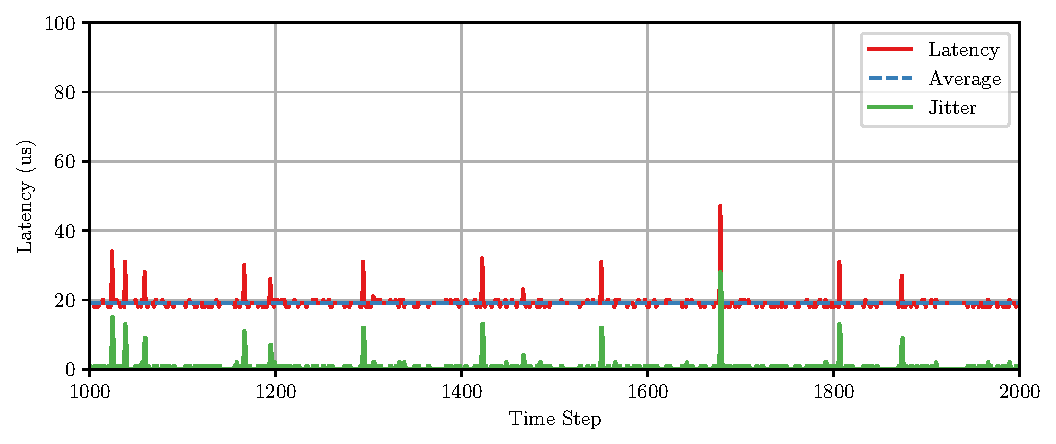
\includegraphics[width=\textwidth]{rt-pi4-mem-times.pdf}
    \caption[Experiment latency graph for shared memory]
    {Experiment latency graph for shared memory}
    \label{fig:rtPi4MemTimes}
\end{figure}

The 

\newpage

\subsection{Sockets}

% present tense
Unix sockets explain

% past tense

\begin{figure}[ht]
    \centering
    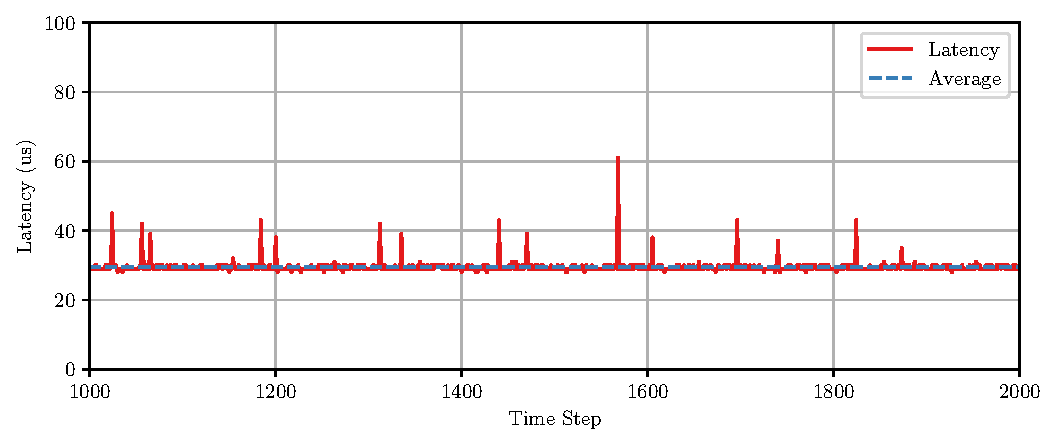
\includegraphics[width=\textwidth]{rt-pi4-socket-times-blocking.pdf}
    \caption[Experiment latency graph for blocking sockets]
    {Experiment latency graph for blocking sockets}
    \label{fig:rtPi4SocketTimesBlocking}
\end{figure}

Although the blocking socket test did perform reasonably well, it was on average over 50\% slower than the shared memory implementation.

\begin{figure}[ht]
    \centering
    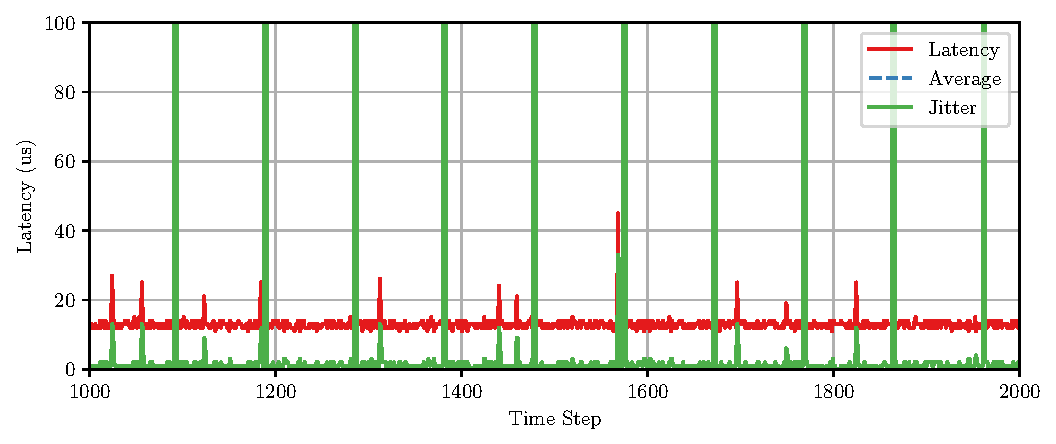
\includegraphics[width=\textwidth]{rt-pi4-socket-times.pdf}
    \caption[Experiment latency graph for non-blocking sockets]
    {Experiment latency graph for non-blocking sockets}
    \label{fig:rtPi4SocketTimes}
\end{figure}

The non-blocking socket performed much better than both the blocking socket and events in shared memory. However, approximately 100 cycles (1 second) significant latencies were introduced at over 40ms, making this solution unviable for a real-time system. It is assumed that these latencies are introduced periodically due to the kernel itself being moved onto the CPU. As the program is busy waiting it never enters the blocked state. Therefore it consumes 100\% of the CPU resources with no opportunity for the kernel to perform management functions.

One possible implementation for the scheduler could use a combination of both the blocking and non blocking sockets. The scheduler could first wakeup a component process using a blocking socket, once on the processor the component can now busy wait for a short period of time on the non blocking socket. Then the scheduler can send the execute command. This reduces the uncertainty of when the process will execute, but overall takes much longer to execute a component as two sequential messages are sent.

To work around this the components could be put into the busy state on alternating processors. So component $a$ could be put into the busy wait and executed, while component $b$ is in the blocked state. These could then be alternated. While this would improve the real-time response of the system, it would unnecessarily consume CPU resources.

\newpage

\subsection{Signalling}

\begin{figure}[ht]
    \centering
    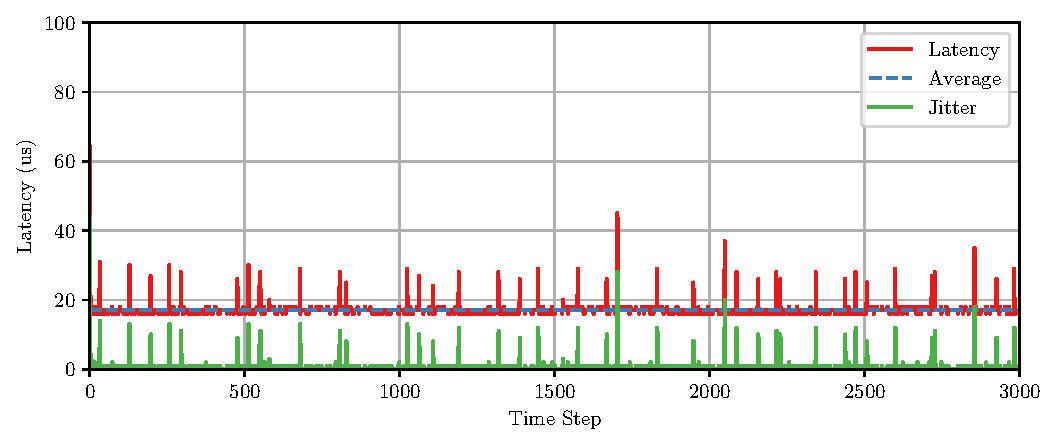
\includegraphics[width=\textwidth]{rt-pi4-signal-times.pdf}
    \caption[Experiment latency graph for signals]
    {Experiment latency graph for signals}
    \label{fig:rtPi4SignalTimes}
\end{figure}

\newpage

\subsection{Evaluation}

\begin{figure}[ht]
    \centering
    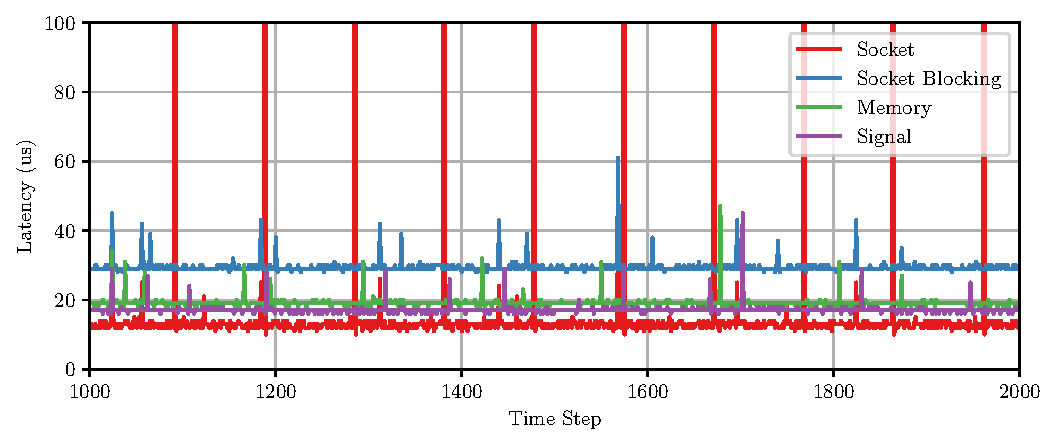
\includegraphics[width=\textwidth]{rt-pi4-compare-times.pdf}
    \caption[Comparison experiment latency graph for all methods]
    {Comparison experiment latency graph for all methods}
    \label{fig:rtPi4CompareTimes}
\end{figure}

\begin{figure}[ht]
    \centering
    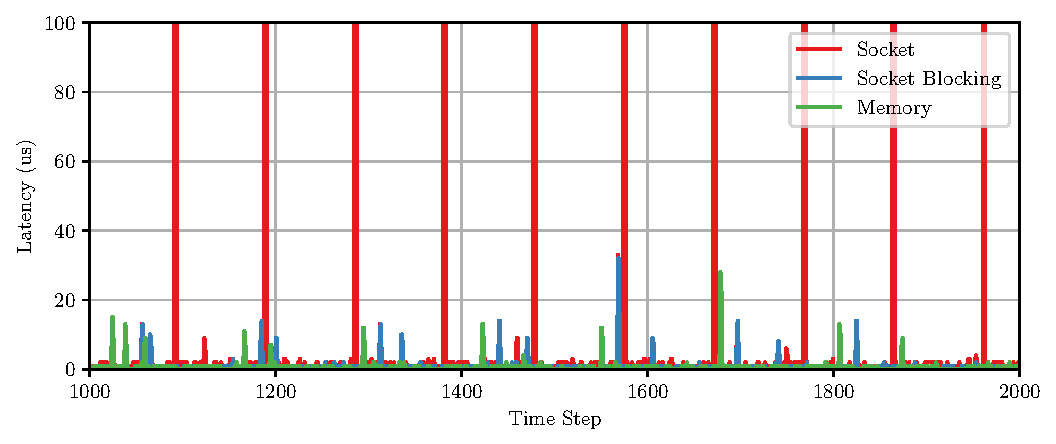
\includegraphics[width=\textwidth]{rt-pi4-compare-times-jitter.pdf}
    \caption[Comparison experiment latency graph for all methods]
    {Comparison experiment jitter graph for all methods}
    \label{fig:rtPi4CompareTimesJitter}
\end{figure}

\subsubsection*{Processor Differences}

% Mention something to do with the Raspberry Pi 5 vs 4 

\begin{figure}[ht]
    \centering
    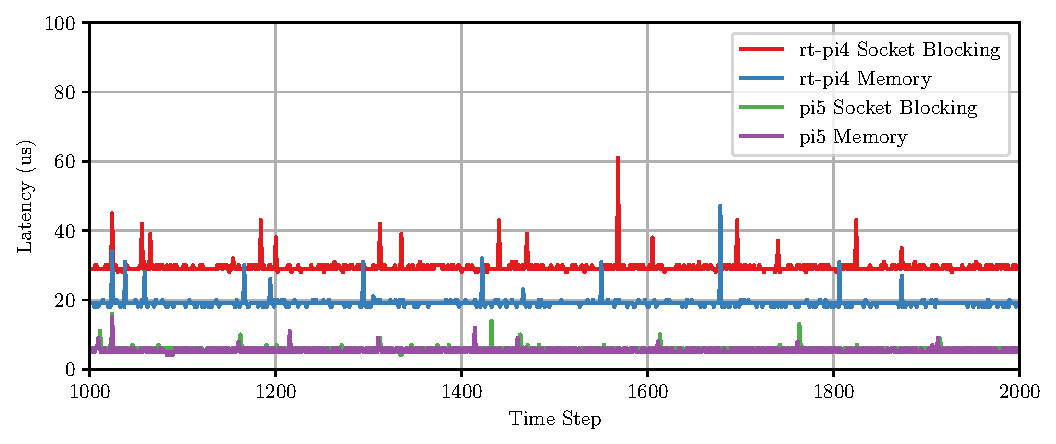
\includegraphics[width=\textwidth]{rt-pi4-vs-pi5.pdf}
    \caption[Comparison experiment latency graph for all methods on Raspberry Pi 4 vs 5]
    {Comparison experiment latency graph for all methods on Raspberry Pi 4 vs 5}
    \label{fig:rtPi4vsPi5CompareTimes}
\end{figure}

\begin{figure}[ht]
    \centering
    \begin{sequencediagram}
        \newinst{r}{Runner}
        \newinst[6]{c}{Component}

        \mess[1]{r}{Execute}{c}
        \mess[1]{c}{Acknowledge}{r}
        \mess{r}{Wake}{c}
        \mess{c}{Acknowledge}{r}

        \stepcounter{seqlevel}

        \mess[1]{r}{Execute}{c}
        \mess[1]{c}{Acknowledge}{r}
        \mess{r}{Wake}{c}
        \mess{c}{Acknowledge}{r}

    \end{sequencediagram}
    \caption{Client-Server messaging}
\end{figure}